\chapter{Модель кровеносной системы и мышечного метаболизма}
\label{chapt:blood_muscle}
\section{Математическая формулировка}
\subsection{Модель кровеносной системы}
Для описания транспорта газов в кровеносной системе используется модель, основанная на разделении системы на пять крупных отделов, соответствующих артериям тканей, головного мозга и легких, системным и легочным венам. В положении равновесия перенос крови между подсистемами осуществляется с постоянной величиной, равной сердечному выбросу. Поток из легочных вен разделяется на две составляющих: потоки в артерии мозга и тканей. Разделение системных артерий на две подсистемы - мозг и ткани связано с различным влиянием газового состава в каждой из данных подсистем на регуляцию дыхания и работы сердца. В данных отделах происходит поглощение кислорода и выделение метаболических излишков углекислого газа. Кровь из артерий мозга и тканей поступает в системные вены, в которых происходит ее перемешивание. Легочные артерии соединены с дыхательной системой. В данном отделе происходит поступление в кровь кислорода из легких и выведение излишков углекислого газа. Для каждой подсистемы рассчитываются осредненные по объему величины, основанные на биохимических реакциях внутри крови.  
  
\begin{figure}[!ht]
\centering
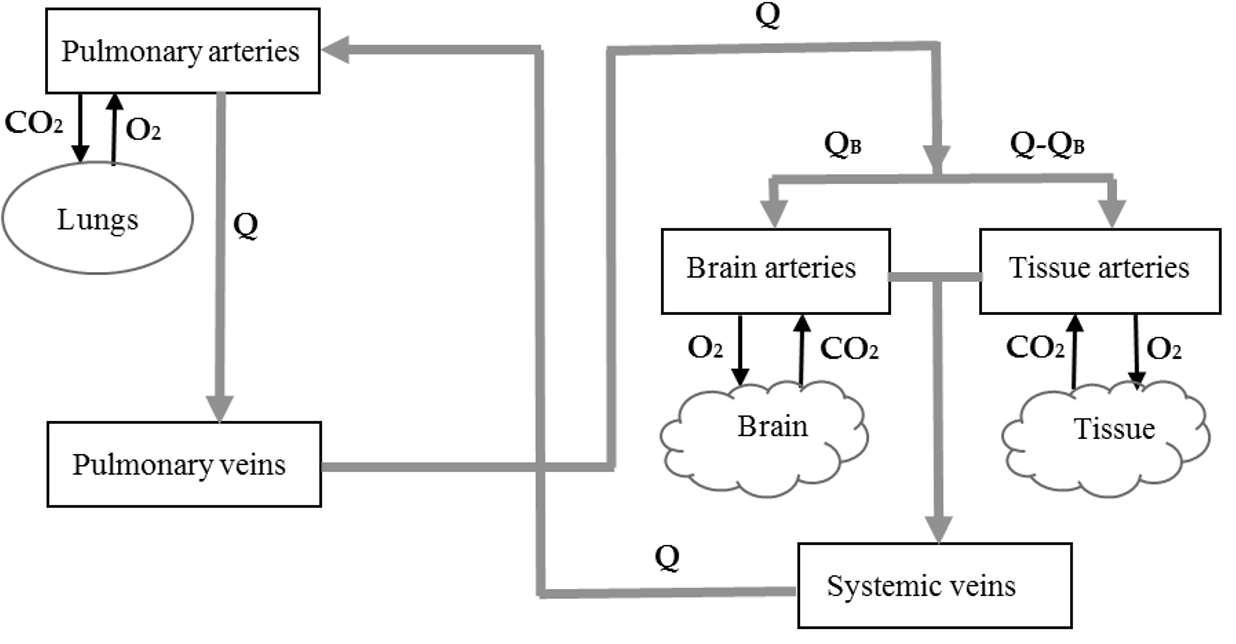
\includegraphics[width=\textwidth]{System}
\caption{Общая схема модели } 
\label{systemChart}
\end{figure}

Кислород переносится кровью в двух формах: растворенном в плазме (примерно 2\%) и в виде химического соединения с гемоглобином (оксигемоглобина).

Оксигемоглобин образуется в результате реакции:
\begin{equation}
Hb+mO_{2} \longleftrightarrow Hb\left(O_{2} \right)_{m}
\label{o2hbreact}
\end{equation}
Где \( 1 \le m \le 4\) ~--- коэффициент оксигенации гемоглобина. В данной работе использовалось значение \( m = 3.6\), полученное эмпирически в \cite{guyton2000}. 

Уравнение суммарной концентрации \( O_{2}\):
\begin{equation}
C_{O_{2}}=C_{O_{2},f}+mC_{Hb_{m}}
\label{hbEq}
\end{equation}
Где \( C_{O_{2,f}}\) ~--- молярная концентрация \( O_{2}\), растворенного в плазме, \( C_{Hb_{m}}\) ~--- молярная концентрация оксигемоглобина.

Суммарная концентрация гемоглобина в крови остается постоянной:
\begin{equation}
T_{Hb}=C_{Hb} + C_{Hb_{m}}
\end{equation}
Где \( C_{Hb}\) ~--- молярная концентрация несвязанного гемоглобина.
Если считать, что реакция (\ref{o2hbreact}) протекает быстро, и достигается состояние квази-равновесия, то:
\begin{equation}
K_{O_{2}}C_{Hb_{m}}=\left(T_{Hb}-C_{Hb_{m}}\right)C_{O_{2,f}}^m,\quad K_{O_{2}}=\frac{k_{O_{2}}^{-}}{k_{O_{2}}^{+}}
\label{o2Hbq}
\end{equation}
Где \( k_{O_{2}}^{+}\)~--- скорость прямой реакции (\ref{o2hbreact}), \( k_{O_{2}}^{-}\)~--- скорость обратной реакции (\ref{o2hbreact})

на основе модели разделения кровеносной системы на подотделы, система уравнений баланса \( O_{2}\) в кровеносной системе принимает вид:
\begin{equation}
\displaystyle \frac{d\mathbf{C_{O_{2}}}}{dt}
=\mathbf{A} \mathbf{C_{O_{2}}}+\begin{pmatrix}
\displaystyle \frac{D_{O_{2}}S}{V_{1}}\left(P_{O_{2},alv}-\frac{C_{O_{2,f},1}}{\sigma_{O_{2}}} \right) \\
0 \\
0 \\
\displaystyle -\frac{\dot{V}_{O_{2},B}}{V_{4}} \\
\displaystyle -\frac{\dot{V}_{O_{2},T}}{V_{5}}
\label{o2Full}
\end{pmatrix}
\end{equation}

\begin{equation}
\mathbf{A}=\begin{pmatrix}
-\frac{Q_{0}}{V_{1}} & 0 & \frac{Q_{0}}{V_{1}} & 0 & 0 \\
\frac{Q_{0}}{V_{2}} & -\frac{Q_{0}}{V_{2}} & 0 & 0 & 0 \\
0 & 0 & -\frac{Q_{0}}{V_{3}} &  \frac{Q_{B}}{V_{3}} &  \frac{Q_{0}-Q_{B}}{V_{3}} \\
0 & \frac{Q_{B}}{V_{4}} & 0 & -\frac{Q_{B}}{V_{4}} & 0 \\
0 & \frac{Q_{0}-Q_{B}}{V_{5}} & 0 & 0 & -\frac{Q_{0}-Q_{B}}{V_{5}} \\
\end{pmatrix}
\end{equation}
Где $\mathbf{C}_{O_2} = \{ C_{O_2},i \}_{i \in [1,..,5]}$, $C_{O_2,i}$ концентрация $O_2$ в $i$-м отделе кровеносной системы (1-легочные артерии, 2-легочные вены, 3-системные вены, 4-артерии головного мозга, 5-системные артерии), \( \sigma_{O_{2}} \) ~--- коэффициент растворимости \( O_{2}\) в крови, \( \dot{V}_{O_{2},B}\) ~---потребление \( O_{2}\) мозгом, \( \dot{V}_{O_{2},T}\) ~---потребление \( O_{2}\) тканями, \( P_{O_{2},alv} \) ~--- парциальное давление \( O_{2}\) в альвеолярном объема, \( V_{i}\)~--- объем \(i\)-го отдела кровеносной системы, \( Q_{0}\) ~---минутный сердечный выброс, \( Q_{B}\) ~---минутный поток крови через артерии головного мозга.

После подстановки в (\ref{o2Full}) уравнений (\ref{hbEq}), (\ref{o2Hbq}) получим:
\begin{equation}
\displaystyle \frac{d\textbf{x}}{dt}
=\mathbf{A} \mathbf{\xi}_{O_{2}}(\textbf{x})+\mathbf{\chi}_{O_{2}}(\textbf{x})
\label{o2Free}
\end{equation}
\begin{equation}
\mathbf{\xi}_{O_{2}}(\mathbf{x})_{i}=\frac{\displaystyle x_{i}+\frac{m T_{Hb}x_{i}^{m}}{ K_{O_{2}}+x_{i}^m}}{S_{O_{2}}(x_{i})}, S_{O_{2}}(x_{i})=1+\frac{m^2K_{O_{2}}T_{Hb}x_{i}^{m-1}}{\left( K_{O_{2}}+x_{i}^m\right)^2}
\end{equation}
\begin{equation}
\mathbf{\chi}_{O_{2}}(\textbf{x})=\begin{pmatrix}
\displaystyle \frac{D_{O_{2}}S}{V_{1}S_{O_{2}}(x_{1})}\left(P_{O_{2},alv}-\frac{x_{1}}{\sigma_{O_{2}}} \right) \\
0 \\
0 \\
\displaystyle -\frac{\dot{V}_{O_{2},B}}{V_{4}S_{O_{2}}(x_{4})} \\
\displaystyle -\frac{\dot{V}_{O_{2},T}}{V_{5}S_{O_{2}}(x_{5})}
\end{pmatrix}
\label{o2source}
\end{equation}

Где \(\mathbf{x}\) вектор состоит из значений \( C_{O_{2,f}}\) в отделах кровеносной системы

\( CO_{2}\) является продуктом окислительного метаболизма в организме. \( CO_{2}\) может переноситься как в составе химических соединений, так и в растворенном виде.

Реакция гидратации молекул \( CO_{2}\) с образованием угольной кислоты и последующей диссоциации на ион бикарбоната и протон:
\begin{equation}
CO_{2}+H_{2} \longleftrightarrow HCO_{3}^{-}+H^{+}
\label{co2react}
\end{equation}
Суммарная концентрация \( CO_{2}\) в крови:
\begin{equation}
C_{CO_{2}}=C_{CO_{2,f}}+C_{HCO_{3}^{-}}
\label{co2freehco3}
\end{equation}
Где \( C_{CO_{2,f}}\) ~--- молярная концентрация \( CO_{2}\), растворенного в крови.

Если считать, что реакция (\ref{co2react}) протекает быстро, и достигается состояние квази-равновесия, то:
\begin{equation}
C_{HCO_{3}^{-}}=K_{CO_{2}}\frac{C_{CO_{2,f}}}{C_{H^{+}}}, \quad K_{CO_{2}}=\frac{k_{CO_{2}}^{-}}{k_{CO_{2}}^{+}}
\label{co2q}
\end{equation}
Где \( k_{CO_{2}}^{+}\)~--- скорость прямой реакции (\ref{co2react}), \( k_{CO_{2}}^{-}\)~--- скорость обратной реакции (\ref{co2react})

Баланс \( HCO_{3}^{-}\) и \( H^{+}\)  в одном отделе кровеносной системы описывается системой уравнений:
\begin{equation}
\frac{dC_{HCO_{3}^{-}}}{dt}=k_{CO_{2}}^{+} C_{CO_{2,f}}-k_{CO_{2}}^{-}C_{H^{+}}C_{HCO_{3}^{-}}+Q_{HCO_{3}^{-}}
\label{hco3Eq}
\end{equation}
\begin{equation}
\frac{dC_{H^{+}}}{dt}=k_{CO_{2}}^{+} C_{CO_{2,f}}-k_{CO_{2}}^{-}C_{H^{+}}C_{HCO_{3}^{-}}+Q_{H^{+}}
\label{hEq}
\end{equation}
Где \( Q_{HCO_{3}^{-}}, Q_{H^{+}}\) ~--- суммарные потоки в/из другие отделы кровеносной системы.

Определим значения $Hc_i$ и $\mathbf{Hc}$: 
\begin{equation}
Hc_{i}=C_{HCO_{3}^{-},i}-C_{H^{+},i}, \mathbf{Hc} = \{ Hc_i \}_{i \in [1,..,5]}
\end{equation}

Из (\ref{hco3Eq}, \ref{hEq}) получаем:
\begin{equation}
\frac{d \textbf{Hc}}{dt}= \mathbf{A Hc}
\label{hhco3Flow}
\end{equation}

Уравнения баланса \(СO_{2}\) в кровеносной системе:
\begin{equation}
\displaystyle \frac{d\mathbf{C_{CO_{2}}}}{dt}
=\mathbf{A} \mathbf{C_{CO_{2}}}+\begin{pmatrix}
\displaystyle \frac{D_{CO_{2}}S}{V_{1}}\left(P_{CO_{2},alv}-\frac{C_{CO_{2,f},1}}{\sigma_{CO_{2}}} \right) \\
0 \\
0 \\
\displaystyle \frac{\dot{V}_{CO_{2},B}}{V_{4}} \\
\displaystyle \frac{\dot{V}_{CO_{2},T}}{V_{5}}
\label{co2Full}
\end{pmatrix}
\end{equation}
Где $\mathbf{C}_{CO_2} = \{ C_{CO_2},i \}_{i \in [1,..,5]}$, $C_{CO_2,i}$ концентрация $CO_2$ в $i$-м отделе кровеносной системы, \( \sigma_{CO_{2}} \) ~--- коэффициент растворимости \( CO_{2}\) в крови, \( \dot{V}_{CO_{2},B}\) ~---выделение \( CO_{2}\) мозгом, \( \dot{V}_{CO_{2},T}\) ~---выделение \( CO_{2}\) тканями, \( P_{CO_{2},alv} \) ~--- парциальное давление \( CO_{2}\) в альвеолярном объеме

После подстановки в (\ref{co2Full}) уравнений(\ref{co2freehco3}), (\ref{co2q}), (\ref{hEq}), (\ref{hhco3Flow}) получим: 
\begin{equation}
\displaystyle \frac{d\textbf{y}}{dt}
=\mathbf{A}\mathbf{\xi}_{CO_{2}}(\textbf{y})+\mathbf{\chi}_{CO_{2}}(\textbf{y})
\label{hco3Flow}
\end{equation}
\begin{equation}
\mathbf{\xi_{CO_{2}}}(\textbf{y})_{i}=\frac{y_{i}^2+(K_{CO_{2}}-Hc_{i})y_{i}}{S_{CO_{2}}(y_{i})K_{CO_{2}}}, S_{CO_{2}}(y_{i})=\frac{K_{CO_{2}}-Hc_{i}+2y_{i}}{K_{CO_{2}}}
\end{equation}
\begin{equation}
\mathbf{\chi_{CO_{2}}}(\mathbf{y})=\begin{pmatrix}
\displaystyle \frac{D_{CO_{2}}S}{V_{1}S_{CO_{2}}(y_{1})}\left(P_{CO_{2},alv}-\frac{y_{1}^2-y_{1}Hc_{1}}{K_{CO_{2}} \sigma_{CO_{2}}} \right) \\
0 \\
0 \\
\displaystyle \frac{\dot{V}_{CO_{2},B}}{V_{4}S_{CO_{2}}(y_{4})} \\
\displaystyle \frac{\dot{V}_{CO_{2},T}}{V_{5}S_{CO_{2}}(y_{5})}
\end{pmatrix}
\label{co2source}
\end{equation}
Где \(\textbf{y}\) вектор состоит из значений $C_{HCO_{3}^{-},i}$.

Изменение газового состава влияет на величину сердечного выброса и перераспределение кровотока между артериями головного мозга и системными артериями. Данный эффект описывается в модели с помощью эмпирических соотношений:
\begin{equation}\label{heartFlow}
Q_{0}=\left(0.937+\frac{0.817}{1+\left(\frac{P_{O_{2},5}}{47.2} \right)^{3.41}} \right)I(P_{CO_{2},5})Q_{MCO},
\end{equation}
\begin{equation}\label{brainFlow}
I(P_{CO_{2},5})=\begin{cases}
1+0.03(P_{CO_{2},5}-40), & N_{CO_{2},5}\le 1 \\
1-0.025(P_{CO_{2},5}-40), & N_{CO_{2},5}> 1 
\end{cases}, 
N_{CO_{2},5}=\frac{P_{CO_{2},5}}{P_{CO_{2},5,0}},
\end{equation}
\begin{equation}
Q_{B}=\left(1.014+\frac{0.734}{1+\left(\frac{P_{CO_{2},5}}{41.4}\right)^{16.6}} \right)\left(0.43+\frac{1.91}{1+10.6e^{-5.25log_{10}P_{CO_{2},5}}} \right)Q_{MCBF},
\end{equation}
Где $Q_{MCO}$  ~---минутный сердечный выброс в покое, $Q_{MCBF}$  ~---минутный кровоток в артерии головного мозга в покое. 

\subsection{Модель мышечного метаболизма}

Напряжение всех физиологических систем спортсмена, обеспечивающих мышечную работу, формирует кислородный запрос, удовлетворяемый работой дыхательной и сердечно-сосудистой систем, показатели которых, при сопоставлении с выполненной механической работой, определяют уровень толерантности организма к физической нагрузке.
Энергия, необходимая для выполнения физического упражнения может быть получена аэробным и анаэробным путем: 
\begin{equation}\label{eq:W}
W=W_{a}+W_{an}
\end{equation}
Где \( W \) ~--- мощность упражнения \( W_{a} \) ~--- мощность, вырабатываемая за счет аэробных источников,  \( W_{an} \) ~--- мощность, вырабатываемая за счет анаэробных источников.

При физических нагрузках небольшой мощности основная часть работы выполняется за счет аэробных источников. Аэробный механизм ресинтеза АТФ включает в основном реакции окислительного фосфорилирования с использованием глюкозы, жирных кислот, белков. Большая часть пирувата, образующегося в результате данной реакции, утилизируется в митохондриях. При этом небольшая часть пиривута преобразуется в лактат и поступает в кровь. В крови поддерживается постоянная концентрация лактата. В зависимости от вклада используемых субстратов окисления и эффективности их трансформации в механическую работу (КПД) можно определить аэробную мощность:
\begin{equation}\label{eq:Wa}
W_{a}=e_{a}\dot{V}_{O_{2},M}
\end{equation}
Где \( \dot{V}_{O_{2},M} \) ~--- мышечный кислородный запрос упражнения, \(e_{a}\) ~--- энергетический эквивалент кислорода.

Повышении мощности физического упражнения приводит к невозможности поддержания скорости синтеза АТФ на необходимом уровне, недостающая часть энергии восполняется за счет анаэробного механизма.

Анаэробный механизм ресинтеза АТФ подразделяется на алактатный и лактатный. Алактатный способ обеспечивает ресинтез АТФ за счет перефосфорилирования между креатинфосфатом и АДФ. При напряженной мышечной деятельности запасы данного источника расходуются достаточно быстро (порядка 10-60 сек.). Лактатный способ основан на ферментативном расщеплении гликогена мышц, а также глюкозы, поступающей из крови, с образованием лактата.  Описываемая математическая модель ориентирована на пролонгированные тренировки, поэтому данный механизм ресинтеза АТФ в дальнейшем не рассматривается. 
Количество выделяемого лактата связано с интенсивностью анаэробных процессов:

\begin{equation}\label{eq:Wan}
W_{an}=e_{la}\dot{V}_{la}
\end{equation}
Где \( \dot{V}_{la} \) ~--- скорость образования лактата, \(e_{la}\) ~--- энергетический эквивалент лактата.

Увеличение концентрации лактата в крови на 1 моль эквивалентно затратам на образование энергии из 3 литров \( O_{2} \) на килограмм массы тела \cite{prampero1999,prampero1981}, поэтому значение энергетического эквивалента лактата \(e_{la}\) взаимосвязана с энергетическим эквивалентом кислорода \(e_{a}\): 
\begin{equation} \label{eq:a_la_eqviv}
e_{la}=\frac{3M}{V_{blood}}e_{a},
\end{equation}
Где \( M \)  ~---масса тела, \(V_{blood}\) ~--- общий объем крови.


Основным механизмом утилизации лактата является окисление в мышцах и миокарде(примерно 60\% от общего объема утилизации). Другая значительная часть (примерно 20\%) утилизируется в печени и кишечнике в результате глюконеогенеза, . Совокупный вклад данных механизмов может быть описан с помощью уравнения реакции первого порядка:
\begin{equation}
\dot{V}_{la,u}=
\begin{cases}
u_{la}\left(C_{la}-C_{la,0}\right), \, C_{la} \geq C_{la,0} \\
0, C_{la} < C_{la,0}
\end{cases},
\label{laUtEq}
\end{equation}
Где \(C_{la} \) ~--- концентрация лактата,\(C_{la,0} \) ~--- концентрация лактата в покое, \(u_{la} \) ~--- скорость утилизации лактата в мышцах, миокарде, печени и кишечнике. \(u_{la} \) неизвестный параметр, который специфичен для каждого отдельного организма.

Часть лактата нейтрализуется буферной системы крови с выделением неметаболического избытка \(CO_{2} \) :
\begin{equation}
\dot{V}_{CO_{2}}=
\begin{cases}
\kappa_{CO_{2}}\left(C_{la}-C_{la,0}\right), \, C_{la} \geq C_{la,0} \\
0, C_{la} < C_{la,0}
\end{cases},
\end{equation}
Где \(\kappa_{CO_{2}} \) ~--- коэффициент неметаболического образования \(CO_{2} \).

Система уравнений для концентраций лактата в кровеносной системе:
\begin{equation}
\frac{d\textbf{z}}{dt}=\textbf{A} \textbf{z}+\mathbf{\chi}_{LA}(\textbf{z})
\label{laEq}
\end{equation}
\begin{equation}
\mathbf{\chi}_{LA}(\textbf{z})=\begin{pmatrix}
0 \\
0 \\
0 \\
0 \\
\displaystyle -u_{la}(z_{5}-C_{la,0})+\frac{\dot{V}_{la}}{V_{5}}
\end{pmatrix}
\end{equation}
Где вектор \(\textbf{z}\) состоит из значений концентрации лактата в отделах кровеносной системы

Лактатный(анаэробный) порог ($W_{LT}$)~--- мощность упражнения, при которой вклад анаэробного метаболизма становится заметным. Данная зависимость определяется безразмерной функцией $\sigma$:
\begin{equation} \label{eq:sigma}
\sigma\left(W\right) = W_{a} / W = 1-\beta e^{\alpha(W-W_{LT})},
\end{equation}
Где $\alpha > 0, 0 < \beta < 1$  ~---неизвестные параметры, который специфичны для каждого отдельного организма. Значение функции $\sigma\left(W\right)$ примерно равно 1 в случае $W < W_{LT}$ и уменьшается в случае $W > W_{LT}$. Значения параметров $\alpha$ и $\beta$ должны быть определены так, что $\sigma\left(W\right) > 0$ для физиологического интервала значений $W$.

Для учета мышечного метаболизма, который описывается уравнениями ($\ref{eq:W}$)-($\ref{eq:sigma}$), уравнения переноса $(\ref{o2source})$ и $(\ref{co2source})$ должны быть модифицированы:
\begin{equation} \label{o2sourceLa}
\mathbf{\chi}_{O_{2}}(\textbf{x})=\begin{pmatrix}
\displaystyle \frac{D_{O_{2}}S}{V_{1}S_{O_{2}}(x_{1})}\left(P_{O_{2},alv}-\frac{x_{1}}{\sigma_{O_{2}}} \right) \\
0 \\
0 \\
\displaystyle -\frac{\dot{V}_{O_{2},B}}{V_{4}S_{O_{2}}(x_{4})} \\
\displaystyle -\frac{1}{V_{5}S_{O_{2}}(x_{5})}\left(\dot{V}_{O_{2},T}+\dot{V}_{O_{2},M}\right)
\end{pmatrix},
\end{equation}

\begin{equation} \label{co2sourceLa}
\mathbf{\chi}_{CO_{2}}(\mathbf{y})=\begin{pmatrix}
\displaystyle \frac{D_{CO_{2}}S}{V_{1}S_{CO_{2}}(y_{1})}\left(P_{CO_{2},alv}-\frac{y_{1}^2-Hc_{1}y_{1}}{K_{CO_{2}} \sigma_{CO_{2}}} \right) \\
0 \\
0 \\
\displaystyle \frac{\dot{V}_{CO_{2},B}}{V_{4}S_{CO_{2}}(y_{4})} \\
\displaystyle \frac{1}{V_{5}S_{CO_{2}}(y_{5})}\left(\dot{V}_{CO_{2},T}+\dot{V}_{O_{2},M}RQ+\kappa_{CO_{2}}\left(z_{5}-C_{la,0}\right) \right)
\end{pmatrix},
\end{equation}
Где $\displaystyle RQ=\frac{\dot{V}_{CO_{2},T}}{\dot{V}_{O_{2},T}}$  ~---дыхательный коэффициент в покое.

Из значения \(e_{a}\) можно оценить эффективность трансформации химической энергии в механическую(КПД):
\begin{equation}\label{eq:kpd}
\eta =\frac{e_{a}}{e_{O_{2}}}
\end{equation}

Если считать, что аэробная энергия вырабатывалась в основном за счет окисления углеводов и жиров, и пропорция данных субстратов во время работы не меняется, то зная величину дыхательного коэффициента в покое \(RQ\) (при окислении только жиров \(RQ=0.7\), только углеводов \(RQ=1\)), можно оценить вклад каждого из субстратов из системы уравнений:
\begin{equation}  \label{eq:CF}
\begin{cases}
\gamma_{C}+0.7\gamma_{F} = RQ  \\
\gamma_{C}+\gamma_{F} = 1
\end{cases},
\end{equation}
Где \(\gamma_{C}\)~--- доля углеводов, \(\gamma_{C}\)~--- доля жиров.

Значения энергетических эквивалентов окисления жиров и углеводов ~\cite{maughan1997} и (\ref{eq:CF}) позволяют получить соотношение:
\begin{equation} \label{eq:e_o2}
e_{O_{2}}=20.9\gamma_{C}+19.5\gamma_{F} \approx 4.7 RQ + 16.23.
\end{equation}
Подставляя (\ref{eq:e_o2}) в (\ref{eq:kpd}) получаем:
\begin{equation}
\eta =\frac{e_{a}}{4.7 RQ + 16.23}.
\end{equation}

\subsection{Общая структура модели}
Модель кровеносной системы и мышечного метаболизма сводится к решению 4х систем ОДУ.

Система ОДУ для концентрации лактата $\mathbf{z} = \{ C_{la,i} \}_{i \in [1,..,5]}$ \eqref{laEq}:
\begin{equation}
\frac{d\textbf{z}}{dt}=\textbf{A}\textbf{z}+\mathbf{\chi}_{LA}(\textbf{z})\notag
\end{equation}
\begin{equation}
\mathbf{\chi}_{LA}(\textbf{z})=\begin{pmatrix}
0 \\
0 \\
0 \\
0 \\
\displaystyle -u_{la}(z_{5}-C_{la,0})+\frac{W_{an}}{e_{la}V_{5}}
\end{pmatrix}\notag
\end{equation}

Система ОДУ для значения $Hc_{i}=C_{HCO_{3}^{-},i}-C_{H^{+},i}, \mathbf{Hc} = \{ Hc_i \}_{i \in [1,..,5]}$ \eqref{hhco3Flow}:
\begin{equation}
\frac{d \textbf{Hc}}{dt}= \mathbf{A Hc} \notag
\end{equation}

Система ОДУ для $CO_{2}$, где $\mathbf{y}=\{ C_{HCO_{3}^{-},i} \}_{i \in [1,..,5]}$ \eqref{co2sourceLa}, \eqref{hco3Flow}  :
\begin{equation}
\displaystyle \frac{d\textbf{y}}{dt}
=\mathbf{A}\mathbf{\xi}_{CO_{2}}(\textbf{y})+\mathbf{\chi}_{CO_{2}}(\textbf{y})\notag
\end{equation}
\begin{equation}
\mathbf{\xi_{CO_{2}}}(\textbf{y})_{i}=\frac{y_{i}^2+(K_{CO_{2}}-Hc_{i})y_{i}}{S_{CO_{2}}(y_{i})K_{CO_{2}}}, S_{CO_{2}}(y_{i})=\frac{K_{CO_{2}}-Hc_{i}+2y_{i}}{K_{CO_{2}}}\notag
\end{equation}
\begin{equation}
\mathbf{\chi}_{CO_{2}}(\mathbf{y})=\begin{pmatrix}
\displaystyle \frac{D_{CO_{2}}S}{V_{1}S_{CO_{2}}(y_{1})}\left(P_{CO_{2},alv}-\frac{y_{1}^2-Hc_{1}y_{1}}{K_{CO_{2}} \sigma_{CO_{2}}} \right) \\
0 \\
0 \\
\displaystyle \frac{\dot{V}_{CO_{2},B}}{V_{4}S_{CO_{2}}(y}_{4)} \\
\displaystyle \frac{1}{V_{5}S_{CO_{2}}(y_{5})}\left(\dot{V}_{CO_{2},T}+\dot{V}_{O_{2},M}RQ+\kappa_{CO_{2}}\left(z_{5}-C_{la,0}\right) \right)
\end{pmatrix} \notag
\end{equation}


Система ОДУ для $O_{2}$, где $\mathbf{x}=\{ C_{O_{2},f,i} \}_{i \in [1,..,5]}$ \eqref{o2sourceLa}, \eqref{o2Free}:
\begin{equation}
\displaystyle \frac{d\textbf{x}}{dt}
=\mathbf{A} \mathbf{\xi}_{O_{2}}(\textbf{x})+\mathbf{\chi}_{O_{2}}(\textbf{x}), S_{O_{2}}(\textbf{x}_{i})=1+\frac{m^2K_{O_{2}}T_{Hb}x_{i}^{m-1}}{\left( K_{O_{2}}+x_{i}^m\right)^2}\notag
\end{equation}
\begin{equation}
\mathbf{\xi}_{O_{2}}(x)_{i}=\frac{\displaystyle x_{i}+\frac{m T_{Hb}x_{i}^{m}}{ K_{O_{2}}+x_{i}^m}}{S_{O_{2}}(x_{i})}\notag
\end{equation}
\begin{equation}
\mathbf{\chi}_{O_{2}}(\textbf{x})=\begin{pmatrix}
\displaystyle \frac{D_{O_{2}}S}{V_{1}S_{O_{2}}(x_{1})}\left(P_{O_{2},alv}-\frac{x_{1}}{\sigma_{O_{2}}} \right) \\
0 \\
0 \\
\displaystyle -\frac{\dot{V}_{O_{2},B}}{V_{4}S_{O_{2}}(x}_{4)} \\
\displaystyle -\frac{1}{V_{5}S_{O_{2}}(x_{5})}\left(\dot{V}_{O_{2},T}+\dot{V}_{O_{2},M}\right)
\end{pmatrix}\notag
\end{equation}

Значения $S, P_{O_{2},alv}, P_{CO_{2},alv}$ определяются из совместного решения с усредненной моделью легких \eqref{AlvEq},\eqref{lungMatter1},\eqref{lungMatter2}:
\begin{equation}
R\frac{dV}{dt}+E(V-V_{0})=P_{g}\sin wt \notag
\end{equation}
\begin{equation}
\frac{d\left(C_{n}V\right)}{dt}  = Q_{n}+D_{n}S\left(P_{n,alv}-\frac{C_{n,1}}{\sigma_{n}}\right)\notag
\end{equation}
\begin{equation}
Q_{n}= \begin{cases} \displaystyle
C_{n}^{air}\frac{dV}{dt}, \frac{dV}{dt} \ge 0 \\
\displaystyle
C_{n}\frac{dV}{dt},  \frac{dV}{dt} <0
\end{cases}\notag
\end{equation}
\begin{equation}
S =\sqrt[{3}]{36\pi \left(V \right)^{2} }\notag
\end{equation}

Эмпирическая модель регуляции сердечного выброса и перераспределения кровотока между  артериями головного мозга и системными артериями \eqref{heartFlow},\eqref{brainFlow}:
\begin{equation}
Q_{0}=\left(0.937+\frac{0.817}{1+\left(\frac{P_{O_{2},5}}{47.2} \right)^{3.41}} \right)I(P_{CO_{2},5})Q_{MCO}\notag
\end{equation}
\begin{equation}
I(P_{CO_{2},5})=\begin{cases}
1+0.03(P_{CO_{2},5}-40), & N_{CO_{2},5}\le 1 \\
1-0.025(P_{CO_{2},5}-40), & N_{CO_{2},5}> 1 
\end{cases}, 
N_{CO_{2},5}=\frac{P_{CO_{2},5}}{P_{CO_{2},5,0}}\notag
\end{equation}
\begin{equation}
Q_{B}=\left(1.014+\frac{0.734}{1+\left(\frac{P_{CO_{2},5}}{41.4}\right)^{16.6}} \right)\left(0.43+\frac{1.91}{1+10.6e^{-5.25log_{10}P_{CO_{2},5}}} \right)Q_{MCBF} \notag
\end{equation}

Эмпирическая модель регуляции дыхания \eqref{VentReg}, \eqref{nVt}:
\begin{equation}
V_{E}=V_{SS}+\left(V_{C}+V_{P}\right)\left(1-e^{-\frac{t}{\tau}}\right) \notag
\end{equation}
\begin{equation}
V_{C}=K_{cCO_{2}}\left(P_{cCO_{2}}-T_{cCO_{2}} \right), V_{C}\ge 0 \notag
\end{equation}
\begin{equation}
V_{P}=K_{pCO_{2}}\left(P_{pCO_{2}}-T_{pCO_{2}} \right)+\left(\frac{570}{P_{pO_{2}}-26.2}-8.05\right)F(P_{pCO_{2}}), V_{P}\ge 0, \notag
\end{equation}
\begin{equation}
F(P_{pCO_{2}})=\begin{cases}
\left(5-4N_{pCO_{2}}^4 \right)^{-1}, & N_{pCO_{2}}\le 1 \\
N_{pCO_{2}}^3, & N_{pCO_{2}}> 1 
\end{cases}, 
N_{pCO_{2}}=\frac{P_{pCO_{2}}}{P_{pCO_{2}}^0} \notag
\end{equation}
\begin{equation}
V_{E}=nV_{T} \notag
\end{equation}
\begin{equation} 
\begin{cases}
n=n_{0},\; V_{T}=\frac{\displaystyle V_{E}}{\displaystyle n_{0}}; & V_{E} \le V_{E,T}  \\
V_{T}=\alpha V_{E}^{\displaystyle \beta},\; n= \frac{\displaystyle V_{E}}{\displaystyle V_{T}}; & V_{E} > V_{E,T}
\end{cases}\notag
\end{equation}

\subsection{Допущения модели}
Модель описывает процессы газообмена, образования и утилизации лактата в осредненном виде. Не выполняется отдельный расчет энергетических процессов в таких важных, с точки зрения спортивной физиологии, органов как сердце, легкие и мышцы. Отдельно не учитывается влияние алактатного синтеза за счет использования запасов креатин-фосфата, поэтому данная модель подходит для пролонгированных упражнений, где его влияние незначительно. Не выполняется разделение механизмов утилизации лактата: окисление в мышцах и миокарде, утилизация в печени и кишечнике в результате глюконеогенеза, нейтрализуется буферной системы крови, выделение с потом и так далее, все процессы объединены в один осредненный. Считалось, что состав субстрата окисления в течении упражнения остается постоянным. Мышцы не рассмотрены как отдельный компартмент, и как следствие не учтено влияние диффузии кислорода в мышцы, влияние миоглобина. Не выполняется моделирование низкоуровневых процессов, например таких цикл Кори и Кребса, лактатный шатл и т.д. Данные упрощения связаны с желанием иметь возможность идентифицировать модель по данным стандартного, нагрузочного тестирования без использования сложных биохимических анализов, миографии и других дополнительных тестов, которые не всегда могут быть выполнены.

\section{Исследование параметров модели при физической нагрузке}
\subsection{Уравнение для лактата}
\label{stabLa}
Уравнение для лактата \eqref{laEq} может быть записано в виде:
\begin{equation}
\frac{d\textbf{z}}{dt}=\textbf{A}\textbf{z}+\mathbf{\chi}_{LA}(\textbf{z})
\end{equation}
\begin{equation}
\mathbf{\chi}_{LA}(\textbf{z})=\begin{pmatrix}
0 \\
0 \\
0 \\
0 \\
\displaystyle -u_{la}(z_{5}-C_{la,0})+\frac{W_{an}}{e_{la}V_{5}}
\end{pmatrix}
\end{equation}

Точки равновесия системы:
\begin{equation}
\textbf{A}\textbf{z}+\mathbf{\chi}_{LA}(\textbf{z})=0
\end{equation}

Существует единственная точка равновесия:
\begin{equation}
\mathbf{z}_{0} = \begin{pmatrix}
C_{la,0}+ \frac{W_{an}}{u_{la}e_{la}V_{5}} \\
C_{la,0}+ \frac{W_{an}}{u_{la}e_{la}V_{5}} \\
C_{la,0}+  \frac{W_{an}}{u_{la}e_{la}V_{5}} \\
C_{la,0}+  \frac{W_{an}}{u_{la}e_{la}V_{5}} \\
C_{la,0}+  \frac{W_{an}}{u_{la}e_{la}V_{5}}
\end{pmatrix}
\end{equation}

Таким образом, физиологически допустимое соотношение между параметрами мышечного метаболизма \(W_{an}, u_{la}, e_{la}\) определяется соотношением:
\begin{equation}
0 \le \displaystyle \frac{W_{an}}{u_{la}e_{la}V_{5}} \le C_{la,max}-C_{la,0}
\end{equation}
где \(C_{la,max}\)~---максимально допустимое содержание лактата в организме.

Тип устойчивости определяется собственными значениями матрицы \(\mathbf{A}\). При физической нагрузке могут регулироваться значения \(Q_{0}, Q_{B}\), остальные значения определяются по антропометрическим показателям. Исследование собственных значений при всех физиологически адекватных значениях показали, что точка \(\mathbf{z}_{0}\) является асимптотически устойчивой по Ляпунову.

\subsection{Уравнение для кислорода в крови}
Уравнение для суммарного содержания \(O_{2}\) в крови \eqref{o2Full} перепишем в виде:
\begin{equation}
\displaystyle \frac{d\mathbf{C}_{O_{2}}}{dt}
=\mathbf{A} \mathbf{C}_{O_{2}}+\begin{pmatrix}
\displaystyle \frac{D_{O_{2}}S}{V_{1}}\left(P_{O_{2},alv}-\frac{x_{1}}{\sigma_{O_{2}}} \right) \\
0 \\
0 \\
\displaystyle -\frac{\dot{V}_{O_{2},B}}{V_{4}} \\
\displaystyle  -\frac{1}{V_{5}}\left(\dot{V}_{O_{2},T}+\dot{V}_{O_{2},M}\right)
\end{pmatrix}
\end{equation}

Точка равновесия:
\begin{equation}
x_{0,1}= \frac{V_{1}\sigma_{O_{2}}}{D_{O_{2}}S}\left(\displaystyle -\frac{\dot{V}_{O_{2},B}}{V_{4}}
\displaystyle  -\frac{1}{V_{5}}\left(\dot{V}_{O_{2},T}+\dot{V}_{O_{2},M}\right)\right)+\sigma_{O_{2}}P_{O_{2},alv} 
\label{equilO2}
\end{equation}

\begin{equation}
A_{0}=x_{0,1}+\frac{mT_{Hb}x_{0,1}^{m}}{K_{O_{2}}+x_{0,1}^{m}}
\end{equation}

\begin{equation}
\displaystyle \mathbf{C}_{O_{2},0}
=\begin{pmatrix}
A_{0} \\
A_{0} \\
A_{0} - \left(\displaystyle \frac{\dot{V}_{O_{2},B}}{V_{4}}
\displaystyle  +\frac{1}{V_{5}}\left(\dot{V}_{O_{2},T}+\dot{V}_{O_{2},M}\right)\right)\frac{V_{1}}{Q_{0}}\\
A_{0}+\frac{\dot{V}_{O_{2},B}}{Q_{0}} \\
A_{0}+\frac{1}{Q_{0}-Q_{B}}\left(\dot{V}_{O_{2},T}+\dot{V}_{O_{2},M}\right)
\end{pmatrix}
\label{equilO2Point}
\end{equation}

При выполнении физической нагрузки лимитирующая возможность организма по доставке \(O_{2}\) к мышцам обусловлена по большей части работой дыхательной системы и сердцем. Из уравнения \eqref{equilO2} можно определить взаимосвязь между усредненным за дыхательный цикл альвеолярным объемом (\(V_{A}\)) и потреблением \(\dot{V}_{O_{2},M}\) мышцами(при этом также используется усредненное за дыхательный цикл значение альвеолярного объема \(P_{O_{2},alv}\)):

\begin{equation}
P_{min} \le  \frac{V_{1}}{D_{O_{2}}\sqrt[{3}]{36\pi \left(V_{A} \right)^{2} }}\left(-\frac{\dot{V}_{O_{2},B}}{V_{4}}
-\frac{1}{V_{5}}\left(\dot{V}_{O_{2},T}+\dot{V}_{O_{2},M}\right)\right)+P_{O_{2},alv} \le P_{max}
\end{equation}

где \(P_{min}, P_{max}\) ~--- минимально и максимально допустимые парциальные давления \(O_{2}\) в организме.

Аналогично из \eqref{equilO2Point} могут быть найдены оценки допустимых соотношений для \(Q_{0}\) и \(Q_{B}\).

\subsection{Уравнение для углекислого газа в крови}
Уравнение для общего содержания \(CO_{2}\) в крови \eqref{co2Full} перепишем в виде:

\begin{equation}
\displaystyle \frac{d\mathbf{C_{CO_{2}}}}{dt}
=\mathbf{A} \mathbf{C_{CO_{2}}}+\begin{pmatrix}
\displaystyle \frac{D_{CO_{2}}S}{V_{1}}\left(P_{CO_{2},alv}-\frac{\mathbf{C}_{O_{2,f},1}}{\sigma_{CO_{2}}} \right) \\
0 \\
0 \\
\displaystyle \frac{\dot{V}_{CO_{2},B}}{V_{4}} \\
\displaystyle \frac{1}{V_{5}}\left(\dot{V}_{O_{2},T}+\dot{V}_{CO_{2},M}RQ+\kappa_{CO_{2}}\left(z_{5}-C_{la,0}\right)\right)
\end{pmatrix}
\end{equation}

Точка равновесия:
\begin{eqnarray}
C_{CO_{2,f},1}= \frac{V_{1}\sigma_{CO_{2}}}{D_{CO_{2}}S{V_{5}}\displaystyle}\left(\dot{V}_{O_{2},T}+\dot{V}_{CO_{2},M}RQ+\kappa_{CO_{2}}\left(z_{5}-C_{la,0}\right)\right)+\\
+\frac{V_{1}\sigma_{CO_{2}}}{D_{CO_{2}}S}\displaystyle \frac{\dot{V}_{CO_{2},B}}{V_{4}}+\displaystyle \sigma_{CO_{2}}P_{CO_{2},alv} \notag
\end{eqnarray}

С учетом соотношение \eqref{co2freehco3}, \eqref{co2q} для \(C_{CO_{2}}, C_{CO_{2,f}}, C_{HCO_{3}^{-}} \) получим:
\begin{equation}
B_{0}=C_{CO_{2,f},1}+\frac{-Hc_{1}+\sqrt{Hc_{1}^{2}+4K_{CO_{2}}C_{CO_{2,f},1}}}{2}
\end{equation}

\begin{equation}
\displaystyle \mathbf{C}_{CO_{2},0}
=\begin{pmatrix}
B_{0} \\
B_{0} \\
B_{0}+\left(\displaystyle \frac{\dot{V}_{CO_{2},B}}{V_{4}} +
    \displaystyle \frac{1}{V_{5}}\left(\dot{V}_{CO_{2},T}+\dot{V}_{O_{2},M}RQ+\kappa_{CO_{2}}\left(z_{0,5}-C_{la,0}\right) \right)\right)\frac{V_{1}}{Q_{0}}\\
B_{0}-\frac{\dot{V}_{CO_{2},B}}{Q_{B}} \\
B_{0}-\frac{1}{Q_{0}-Q_{B}}\left(\dot{V}_{CO_{2},T}+\dot{V}_{O_{2},M}RQ+\kappa_{CO_{2}}\left(z_{0,5}-C_{la,0}\right) \right)
\end{pmatrix}
\end{equation}

При выполнении физической нагрузки лимитирующая возможность организма по выведению излишков \(CO_{2}\) также  обусловлена работой дыхательной системы и сердцем, но, в отличии от \(O_{2}\), дополнительный вклад дает работа буферных систем (\(\kappa_{CO_{2}}\)). При этом необходимо использовать точку равновесия \(\mathbf{z}_{0,5}\) из п.\ref{stabLa}.



\section{Численные методы}
\label{sec:bloodNumeric}

\subsection{Расчет уравнений переноса в кровеносной системе}
Модель кровеносной системы сводится к последовательному решению четырех задач Коши для систем ОДУ вида:

\begin{equation} \label{eq:Koshi}
\frac{d\mathbf{x}(t)}{dt}=\mathbf{f}(t,\mathbf{x}(t)), \, \mathbf{x}(0)=\mathbf{x_0}.
\end{equation}

Система №1: (\ref{laEq}) описывает образование, утилизацию и транспорт лактата.  Система №2: (\ref{o2Free})-(\ref{o2source}) описывает транспорт кислорода. Системы №3: (\ref{hhco3Flow}) и №4: (\ref{hco3Flow})-(\ref{co2source}) описывают транспорт углекислого газа.

Коэффициент жесткости системы:
\begin{equation}
    \zeta = \frac{\max \limits_{Re \, \lambda_k < 0} \mid Re \, \lambda_k \mid}{\min \limits_{Re \, \lambda_k < 0} \mid Re \, \lambda_k \mid},
\end{equation}

где $\lambda_k$~---собственные значения матрицы Якоби $\displaystyle \mathbf{f}_\mathbf{x} = \left\{ \frac{\partial \mathbf{f}}{\partial \mathbf{x}} \right\}$, $\mathbf{f}(t,\mathbf{x}(t))$~--- правая часть(\ref{eq:Koshi})
Значения $\lambda_k$ были численно определены при физиологическом диапазоне входных параметров. Эксперименты показали, что для системы №1: \(\zeta \sim 10\), для системы №2: \(\zeta \sim 10^{4}\), для системы №3: \(\zeta \sim 10\), для системы №4: \(\zeta \sim 10^{5}\). Таким образом система уравнений для кровеносной системы является жесткой и необходимо применение специальных численных методов.

Для решения жестких систем ОДУ использовался неявный одношаговый A,L - устойчивый метод третьего порядка аппроксимации из семейства схем Обрешкова \cite{Hairer1999}.

Для системы ОДУ запишем одношаговый метод в общем виде с использованием метода неопределенных коэффициентов:

\begin{equation}
\sum_{k=0}^{1}\left[a_{k}\mathbf{x}^{n+k}-\tau b_{k}\mathbf{x}_{t}\left(t^{n+k}+k\tau, \mathbf{x}^{n+k}\right)-\tau^{2}c_{k}\mathbf{x}_{tt}\left(t^{n+k}+k\tau,\mathbf{x}^{n+k}\right)\right]=0
\end{equation}

Дифференцируем правую и левую часть исходной системы по t:
\begin{equation}
\mathbf{x}_{tt}=\frac{\partial \mathbf{f}}{\partial t}+\mathbf{f}_{x}\mathbf{f}
\end{equation}

После подстановки получаем:
\begin{equation}
\sum_{k=0}^{1}\left[a_{k}\mathbf{x}^{n+k}-\tau b_{k}\mathbf{f}^{n+k}-\tau^{2}c_{k}\left(\frac{\partial \mathbf{f}^{n+k}}{\partial t}+\mathbf{f}_{x}^{n+k}\mathbf{f}^{n+k}\right)\right]=0
\end{equation}

Для получения третьего порядка точности необходимо выбрать следующие значения коэффициентов:
\begin{equation}
a_{1}=1, a_{0}=-1, c_{0}=0, c_{1}=c_{0}-\frac{1}{6},
b_{0}=\frac{1}{2}+c_{0}+c_{1}, b_{1}=\frac{1}{2}-c_{0}-c_{1}
\end{equation}

Значение \( x^{n+1}\) на верхнем временном слое $t_{n+1} = t_n+\tau$ может быть найдено из нелинейной системы уравнений:

\begin{equation}
\mathbf{R}\left(\mathbf{x}^{n+1}\right)=\mathbf{r}^{n}+a_{1}\mathbf{x}^{n+1}-\tau b_{1}\mathbf{f}^{n+1}-\tau^{2}c_{1}\left[\frac{\partial\mathbf{f}^{n+1}}{\partial t}+\mathbf{f}_{x}^{n+1}\mathbf{f}^{n+1}\right]=0
\end{equation}

где

\begin{equation}
\mathbf{r}^{n}=a_{0}\mathbf{x}^{n}-\tau b_{0}\mathbf{f}^{n}-\tau^{2}c_{0}\left[\frac{\partial\mathbf{f}^{n}}{\partial t}+\mathbf{f}_{x}^{n}\mathbf{f}^{n}\right]
\end{equation}

Система может быть решена итерационным методом Ньютона:
\begin{equation}\label{eq:iter_Obreshkov}
\mathbf{x}_{s+1}^{n+1}=\mathbf{x}_{s}^{n+1}-\mathbf{B}^{-1}\left(t^{n+k}, \mathbf{x}_{s}^{n+1}\right)\mathbf{R}\left(\mathbf{x}_{s}^{n+1}\right)
\end{equation}

где $s$~---индекс итерации

\begin{equation}
\mathbf{B}=\frac{\partial\mathbf{R}}{\partial\mathbf{x}^{n+1}}=E-\tau b_{1}\mathbf{f}_{x}-\tau^{2}c_{1}\left[\frac{\partial}{\partial \mathbf{x}}\left(\frac{\partial\mathbf{f}}{\partial t}\right)+\mathbf{f}_{x}\mathbf{f}_{x}+\mathbf{C}\right]
\end{equation}

где \(\mathbf{E}\) ~--- единичная матрица, \(\mathbf{C}\) ~--- матрица, столбцами которой являются векторы \(\mathbf{f}\displaystyle\frac{\partial \mathbf{f}_{x}}{\partial x_{i}}\).

Итерации (\ref{eq:iter_Obreshkov}) повторяются до достижения критерия сходимости
\begin{equation}
\frac{\left|\mathbf{x}_{s+1}^{n+1}-\mathbf{x}_{s}^{n+1}\right|}{\mathbf{x}_{s}^{n+1}} < \varepsilon
\end{equation}

Где $\varepsilon=10^{-6}$.
\subsection{Совместный расчет уравнений дыхательной и кровеносной систем}

В данном разделе описан алгоритм проведения совместных численных расчетов транспорта газов в дыхательной и кровеносной системах \cite{GolovCmodel2017}. На каждом временном шаге (при расчетах использовалось значение $\tau=10^{-2}$~сек) до достижения критерия сходимости выполнялась итерационная процедура, включающая блоки расчета мышечного метаболизма, системных величин (дыхательный объем, объем легких, сердечный выброс и т.д.), баланса газов ($O_2, CO_2$) и лактата в крови.

\begin{enumerate}
	
	\item {\bf Мышечный метаболизм.}

\begin{enumerate}
	
	\item \label{it:iter_start} Доля аэробного энергопотребления ($\sigma$) рассчитывается из~\eqref{eq:sigma}. Уровень потребления кислорода ($\dot{V}_{O_{2},M}$), который необходим для аэробного метаболизма в мышцах, рассчитывается из~\eqref{eq:Wa}. 
	
	\item Уровень производства лактата ($\dot{V}_{la}$) в следствии анаэробного метаболизма рассчитывается из~\eqref{eq:Wan}.
	
\end{enumerate}	

	\item {\bf Системные величины.}

\begin{enumerate}
		
	\item Дыхательный объем $V_{T}$ и количество дыхательных циклов в минуту $n$ рассчитываются из (\ref{nVt}). 
	
	\item Минутный  $Q_{0}$ и минутный поток крови в артерии головного мозга $Q_{B}$ рассчитываются из \eqref{heartFlow}, \eqref{brainFlow}. 
	
	\item Объем легких $V(t)$ рассчитывается из (\ref{V_analyt}). Текущие альвеолярные концентрации $O_{2}$ и $CO_{2}$ рассчитываются из \eqref{lungMatter1}.   

\end{enumerate}

	\item {\bf Баланс газов и лактата в крови.}

\begin{enumerate}	
	
	\item Определяются вектора начальных значений:
	\begin{equation*}
	\tilde{\mathbf{x}}^{n+1} = \mathbf{x}^{n}, \tilde{\mathbf{y}}^{n+1} = \mathbf{y}^{n}, \tilde{\mathbf{z}}^{n+1} = \mathbf{z}^{n}, \mathbf{\tilde{H}c}^{n+1} = \mathbf{Hc}^{n}, 
	\end{equation*}
	где $\tilde{\mathbf{x}}^{n+1}$, $\tilde{\mathbf{y}}^{n+1}$, $\tilde{\mathbf{z}}^{n+1}$, $\tilde{\mathbf{Hc}}^{n+1}$ текущие значения векторов концентраций соответствующих веществ в отделах кровеносной системы.
	
	\item Значение $\tilde{\mathbf{z}}^{n+1}$ рассчитывается из системы (\ref{laEq}).
	%Task~1.
	% $\widetilde{C}_{La}^{n+1}$.
	
	\item Значение $\tilde{\mathbf{x}}^{n+1}$ рассчитывается из системы (\ref{o2Free}).
	%Task~2. 
	% $\widetilde{C}_{O_{2,f}}^{n+1}$. 
	
	\item Значение $\mathbf{\widetilde{H}c}^{n+1}$ рассчитывается из системы (\ref{hhco3Flow}).
	% Task~3. 
	% $\widetilde{C}_{Hc}^{n+1}$
	
	\item Значение $\tilde{\mathbf{y}}^{n+1}$ рассчитывается из системы (\ref{hco3Flow}) с использованием значений $\tilde{\mathbf{x}}^{n+1}$, $\tilde{\mathbf{z}}^{n+1}$, $\mathbf{\widetilde{H}c}^{n+1}$.
	% Task~4. 

\end{enumerate}

	\item {\bf Проверка критерия сходимости алгоритма.}
	
	 Критерий сходимости, при удовлетворении которого итерационная процедура останавливается:
	\begin{equation*}
	\delta \left( \tilde{\mathbf{x}}^{n+1}, \mathbf{x}^{n+1} \right) < \varepsilon, \delta \left( \tilde{\mathbf{y}}^{n+1}, \mathbf{y}^{n+1} \right) < \varepsilon, \delta \left( \tilde{\mathbf{z}}^{n+1}, \mathbf{z}^{n+1} \right) < \varepsilon, \delta \left( \mathbf{\tilde{H}c}^{n+1}, \mathbf{Hc}^{n+1} \right) < \varepsilon,
	\end{equation*}
	Где $\delta \left( \tilde{\mathbf{s}}^{n+1}, \mathbf{s}^{n+1} \right) = \displaystyle \frac{\|\tilde{\mathbf{s}}^{n+1} - \mathbf{s}^{n+1}\|}{\|\mathbf{s}^{n+1}\|}$, $\|\mathbf{s}\| = \max \limits_j \left| s_j \right|$; $\tilde{\mathbf{s}}^{n+1}$, $\mathbf{s}^{n+1}$, $\mathbf{s}$ вектора одинаковой размерности. 
	
	Иначе итерационная процедура продолжается с новыми значениями:
	\begin{equation*}
	{\mathbf{x}}^{n+1} = \tilde{\mathbf{x}}^{n+1}, \mathbf{y}^{n+1} = \tilde{\mathbf{y}}^{n+1}, \mathbf{z}^{n+1} = \tilde{\mathbf{z}}^{n+1}, \mathbf{Hc}^{n+1} = \mathbf{\tilde{H}c}^{n+1}.
	\end{equation*}

\end{enumerate}

\subsection{Идентификация параметров модели мышечного метаболизма}
Параметры модели мышечного метаболизма: \(e_{a}, u_{la}, \kappa_{CO_{2}}\), $\beta$, $\alpha$ могут сильно отличаться для каждого человека. При этом корректное определение значений данных параметров очень сильно влияет на точность результатов модели. Остальные значения параметров модели могут быть взяты, как средние по популяции, либо с использование алло-метрических показателей на основе роста и веса.  

Неизвестные параметры могут быть идентифицированы по результатам физиологических нагрузочных тестов, во время которых регистрируются показатели потребления \(O_{2}\), выделения \(СO_{2}\), минутной вентиляции легких \(V_{E}\), и концентрации лактата (LA). 
Оптимальные значения параметров мышечного метаболизма $e_{a}$, $u_{la}$, $\kappa_{CO_{2}}$, $\beta$, $\alpha$ определялись из минимизации функционала:
\begin{equation} \label{eq:functional}
\Phi = \sum \limits_{M \in \{O_2, CO_2, V_E, LA\}} \left( \frac{1}{N_M}\sum_{i=1}^{N_M} huber\left(\Delta_{M,i}\right) \right),
\end{equation}
\noindent Где
\begin{equation} \label{eq:huber}
huber(\Delta)=\begin{cases}
\frac{1}{2}\Delta^2,& |\Delta| \le \delta\\
\delta(|\Delta|-\frac{1}{2}\delta),& |\Delta| > \delta
\end{cases}, 
\Delta_{M,i}=\frac{x_{M,i}^{exp}-x_{M,i}^{num}}{x_{M,i}^{exp}}, \delta_M = 1.5\sqrt{\frac{1}{N_M}\sum_{i=1}^{N_M}\Delta_{M, i}^{2}},
\end{equation}
\noindent $M$~---индекс параметра (($O_{2}$)- объем потребления $O_{2}$, ($CO_2$)- объем выделения $CO_{2}$, ($LA$)- концентрация лактата в крови , ($V_E$)- минутная вентиляция легких ), $N_M$~--- количество экспериментальных измерений параметра $M$, $x_{M,i}^{exp}$ ~--- $i$-ое измерение значения параметра $M$, $x_{M,i}^{num}$ ~--- $i$-ое расчетное значение параметра $M$.

Использование функции Хьюбера обусловлено тем, что экспериментальные данные могут быть зашумлены и иметь выбросы, которые сильно влияют на результат. 

Функционал (\ref{eq:functional}) не является выпуклым, поэтому для решения задачи применялись алгоритмы глобальной оптимизации. Было рассмотрено два наиболее популярных алгоритма, реализованных в библиотеке scipy.optimize:

1) Basin-hopping \cite{Wales1997}- стохастический алгоритм, основанный на идее мулти-старта со случайным выбором начальных точек и поиском локального минимума в каждой из этих точек. В качестве алгоритмов локальной оптимизации использовались методы: 'BFGS', 'L-BFGS', 'Nelder-Mead', 'Powell'.    

2) Алгоритм дифференциальной эволюции \cite{Storn1997} - стохастический алгоритм, в котором сначала генерируется случайный набор(поколение) значений(особей). На каждой итерации алгоритм генерирует новое поколение векторов, случайным образом комбинируя векторы из предыдущего поколения (операция "скрещивания" и "мутации"). Итерации выполняются до достижения сходимости. Значения оптимизируемых параметров $e_{a}$, $u_{la}$, $\kappa_{CO_{2}}$, $\alpha$, $\beta$ выбирались из промежутков $e_{a}\in [0.1e_{O_{2}}, 0.4e_{O_{2}}]$, 
$u_{la}\in [10^{-4}, 10^{-2}]$, 
$\kappa_{CO_{2}}\in [10^{-1}, 10]$, 
$\beta \in [10^{-3}, 10^{-1}], \alpha\in [10^{-3}, 10^{-1}]$. 

Численные эксперименты показали, что базовая версия алгоритма дифференциальной эволюции требуют на порядок меньше вычислений целевой функции по сравнению с настроенным алгоритмом Basin-hopping при одинаковой точности решения. Поэтому дальнейшие исследования были связаны с настройкой алгоритма дифференциальной эволюции.

Вариации алгоритма дифференциальной эволюции связаны с выбором параметров x/y/z . 

x ~-- определяет вектор, для которого будет выполнена операция мутации. 'rand'~-- выбор случайного вектора, 'best' ~-- выбор вектора с минимальным функционалом для текущей популяции.

y ~-- количество разностных векторов.

z ~-- схема операции кроссовера. 'bin' ~-- независимые биномиальные эксперименты.

Было протестировано четыре наиболее популярных схемы 'best/1/bin','rand/1/bin','best/2/bin','rand/2/bin', результаты показаны в таблице \ref{tab:opt}. 

\begin{table}[!ht]
\centering
\caption{Характерная зависимость количества расчетов целевого функционала до достижения сходимости от выбора схемы алгоритма дифференциальной эволюции }
\medskip
\begin{tabular}{|c|c|}
\hline
Схема  & Кол-во расчетов \\
\hline
'best/1/bin' & 1260 \\
\hline
'rand/1/bin' & 1569 \\
\hline
'best/2/bin' & 1701  \\
\hline
'rand/2/bin' & 1704  \\
\hline
\end{tabular}
\label{tab:opt}
\end{table}

Таким образом, для задачи идентификации параметров модели наилучшими свойствами обладает схема 'best/1/bin'. 

\subsection{Алгоритм определения анаэробного порога}
В модели мышечного метаболизма используется значение анаэробного порога. Корректность определения анаэробного порога во многом влияет на точность модели. 

Значение анаэробного порога (ПАНО) может быть определено с помощью теста с возрастающей физической нагрузкой. Во время тестирования регистрируются показатели, получаемые неинвазивными методами: потребление кислорода, выделение углекислого газа, легочная вентиляция, частота сердечных сокращений и показатель, получаемый инвазивным методом - концентрация лактата в капиллярной крови. Наиболее полную информацию дают тесты с повышающейся нагрузкой по линейному и ступенчатому протоколам, в которых практически достигается уровень максимального потребления кислорода и максимальное утомление \cite{bel2005}.

На результаты тестирования могут влиять физиологическое и психологическое состояние человека, предшествующие физические нагрузки, время и состав принимаемой пищи в день теста, характер предварительной разминки \cite{Burnley2002}. В связи с этим, спортсмен получает инструкции, соблюдение которых стандартизирует условия проведения тестирования по всем перечисленным пунктам. 

Разворачивание физиологических процессов при возрастающей мощности нагрузки состоит из 3-х фаз, которые в динамике представляют собой кривые физиологических показателей с характерными переходными участками, которые могут быть аппроксимированы кусочно-линейными отрезками. Энергетическое обеспечение в первой фазе осуществляется полностью за счет аэробных метаболических процессов. Первая точка излома называется «аэробным порогом» и начинает вторую фазу, при которой образование лактата в скелетной мышце превышает его распад и начинает постепенно накапливаться. Третья фаза начинается вторым изломом, который называется «порог анаэробного обмена» и, согласно, представляет собой критический режим работы, при котором происходит переход от преимущественно аэробного энергообеспечения мышечной работы к смешанному энергообразованию с нарастающим участием анаэробного гликолиза, сопровождающимся быстрым накоплением лактата в работающих мышцах и крови.
Основной проблемой в определении АэП и ПАНО является идентификация значений точек перегибов кусочно-линейных кривых физиологических показателей, которые вследствие наличия шума в данных, не могут быть определены с высокой точностью. 

В тестах с возрастающей нагрузкой до отказа временные ряды показателей VCO2(t) (выделение углекислого газа), RER(t) (отношение потребления кислорода к выделению углекислого газа), VE(t) (минутная вентиляция легких), ExсCO2(t) (дополнительное выделение углекислого газа по сравнению с состоянием покоя) могут быть описаны уравнением регрессии:
\begin{equation}
y(t)=x(t)+\varepsilon(t)
\end{equation}
где \(x(t)\) ~--- кусочно-линейная функция, \(\varepsilon(t)\) ~--- погрешность измерений

В уравнение регрессии показателя ExсСО2, состоящей из 2-х частей, присутствует одна точка перегиба. Уравнения регрессии показателей VCO2, RER, VE состоят из 3-х кусочно-линейных участков и имеют две точки перегиба. 
Для каждого сопряжения кусочно-линейных участков справедливо соотношение:

\begin{equation}
y=\begin{cases}
y_{1}+b_{1}(x_{i}-x_{1}), & x_{i} < x_{2} \\
y_{2}+b_{2}(x_{i}-x_{2}), & x_{2} \le x_{i} < x_{3} \\
y_{3}+b_{3}(x_{i}-x_{3}), & x_{3} < x_{i} 
\end{cases}
\end{equation}
\begin{gather}
y_{2}=y_{1}+b_{1}(x_{2}-x_{1}) \notag \\
y_{3}=y_{2}+b_{2}(x_{3}-x_{2}) \notag
\end{gather}
где \(x_{1}\) ~--- начало выполнения теста, \(x_{2}\) ~--- АэП, \(x_{3}\) ~--- ПАНО 

При проведении нагрузочных тестов присутствует погрешность измерения не только \(y_{i}\), но и \(x_{i}\). Для повышения точности определения изгиба кривых используется метод ортогональной регрессии. В этом случае функция суммы квадратов ошибок принимает вид:

\begin{eqnarray}
S=\sum_{i=0}^m \frac{\left(y_{1}+b_{1}(x_{i}-x_{1})-y_{i} \right)^{2}}{b_{1}^{2}+1} + \\
+\sum_{i=m+1}^k \frac{\left(y_{2}+b_{2}(x_{i}-x_{2})-y_{i} \right)^{2}}{b_{2}^{2}+1}+ \notag\\
+\sum_{i=k+1}^N \frac{\left(y_{3}+b_{3}(x_{i}-x_{3})-y_{i} \right)^{2}}{b_{3}^{2}+1} \notag
\end{eqnarray}

Параметры \(b_{1}, b_{2}, y_{1}, x_{2}, x_{3}\) определяются из численного решения задачи глобальной оптимизации.

Устойчивость получаемого решения к малым изменениям показателя повышалась с использованием специальной процедуры робастного оценивания \cite{huber1984}. 

Оценка стандартной ошибки наблюдения \((x_{i}, y_{i})\) , получаемая из решения оптимизационной задачи \cite{Boggs1988}.

Если \(|r_{i}|>c\sqrt{S}\), то выполняется корректировка:

\begin{equation}
r_{i}=\frac{y_{0}+b(x_{i}-x_{0})-y_{i}}{\sqrt{b^{2}+1}}
\end{equation}

Крайние значения наблюдений \((x_{i}, y_{i})\) корректируются заменой на значения их псевдонаблюдений: 
\begin{equation}
r'_{i}=\begin{cases}
r_{i}-c\sqrt{S},& r_{i}>0 \\
r_{i}+c\sqrt{S},& r_{i}<0
\end{cases}
\end{equation}

\begin{equation}
x'_{i}=\frac{r'_{i}b}{\sqrt{b^{2}+1}}+\frac{(y_{i}-y_{0}+bx_{0})b+x_{i}}{b^{2}+1}
\end{equation}

\begin{equation}
y'_{i}=-\frac{1}{b}(x'_{i}-x_{i})+y_{i}
\end{equation}

Константа c регулирует степень робастности. Далее по псевдо- наблюдениям \((\hat{x}_{i}, \hat{y}_{i})\)  вычисляются новые значения   подгонки \((x_{i}, y_{i})\). Действия повторяются до достижения сходимости.

\begin{figure}[!ht]
	\centering
	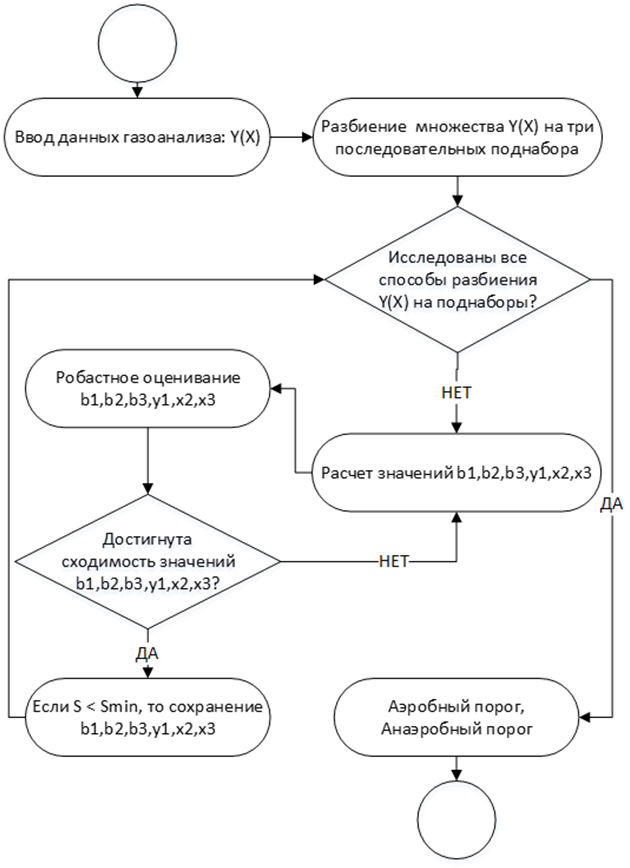
\includegraphics[scale=0.6]{sportAlg.png}
	\caption{Алгоритм расчета параметров робастной кусочно-линейной регрессии } 
\end{figure}

Для значения каждого параметра модели может быть выполнен расчет доверительного интервала (ДИ). Расчет ДИ выполняется с помощью модифицированного для временных серий метода бутстреппинга \cite{efron1988}~--- the moving block bootstrap(MBB): 

Пусть $\{X_{1},...,X_{n}\} \equiv \mathbf{X_{n}}$~--- временной ряд. Пусть $l$ ~---целое число: $1\le l<n$. Определим пересекающиеся блоки $\mathcal{B}_{1},...,\mathcal{B}_{n-l+1}$ длинны $l$, принадлежащие $\mathbf{X_{n}}$:

$\mathcal{B}_{1}=(X_{1},X_{2},...,X_{l})$,

...

$\mathcal{B}_{n-l+1}=(X_{n-l+1},...,X_{n})$.

Таким образом, на основе временного ряда для показателей газоанализа одного нагрузочного теста генерируется множество псевдо-выборок того же размера,
состоящих из случайной комбинаций $n/l$ блоков $\mathcal{B}$, при этом используется алгоритм случайного выбора с возвращением.

Пусть \(p_{i}\), где \(i=1..n\) ~-- расчетное значение параметра модели для каждой псевдо-выборки. Тогда

\begin{equation}
E(p)=\frac{1}{n}\sum_{i=1}^n p_{i}
\end{equation}

\begin{equation}
SE_{boot}(p)=\sqrt{\frac{1}{n-1}\sum_{i=1}^{n}\left(p_{i}-E(p)\right)^{2}}
\end{equation}

\begin{equation}
CI_{\gamma} = \left[E(p)-t_{\gamma,n}SE_{boot}(p), E(p)+t_{\gamma,n}SE_{boot}(p)\right]
\end{equation}
где \(E(p)\) ~-- среднее значение расчетного значения параметра \(p\), \(SE_{boot}(p)\) ~-- стандартная ошибка метода бутстреппинга, \(CI_{\gamma}\) ~-- доверительный интервал оценки параметра p, \(t_{\gamma,n}\) ~-- критическое значение \(\gamma\)-го квантиля распределения Стьюдента \(t(\gamma, n-1)\).

АэП и ПАНО определяются. как среднее значение ДИ по всем показателям газоанализа \cite{GolovIt2017}.

\section{Программный комплекс}
Для программной реализации модель кровеносной системы и мышечного метаболизма использовался абстрактная модель и архитектура, описанная в разделе \ref{lung:soft}. Для расчета 900 сек. нагрузочного теста на двух ядерном Intel Core i3-2100 3.10GHz, Windows 7-64, 16Gb RAM требовалось в среднем 10 секунд. 

Для идентификации параметров модели по данным нагрузочного тестирования программный комплекс был дополнен модулем оптимизации (Рис.~\ref{fig:soft_muscle}). 
\begin{figure}[!ht]
	\centering
	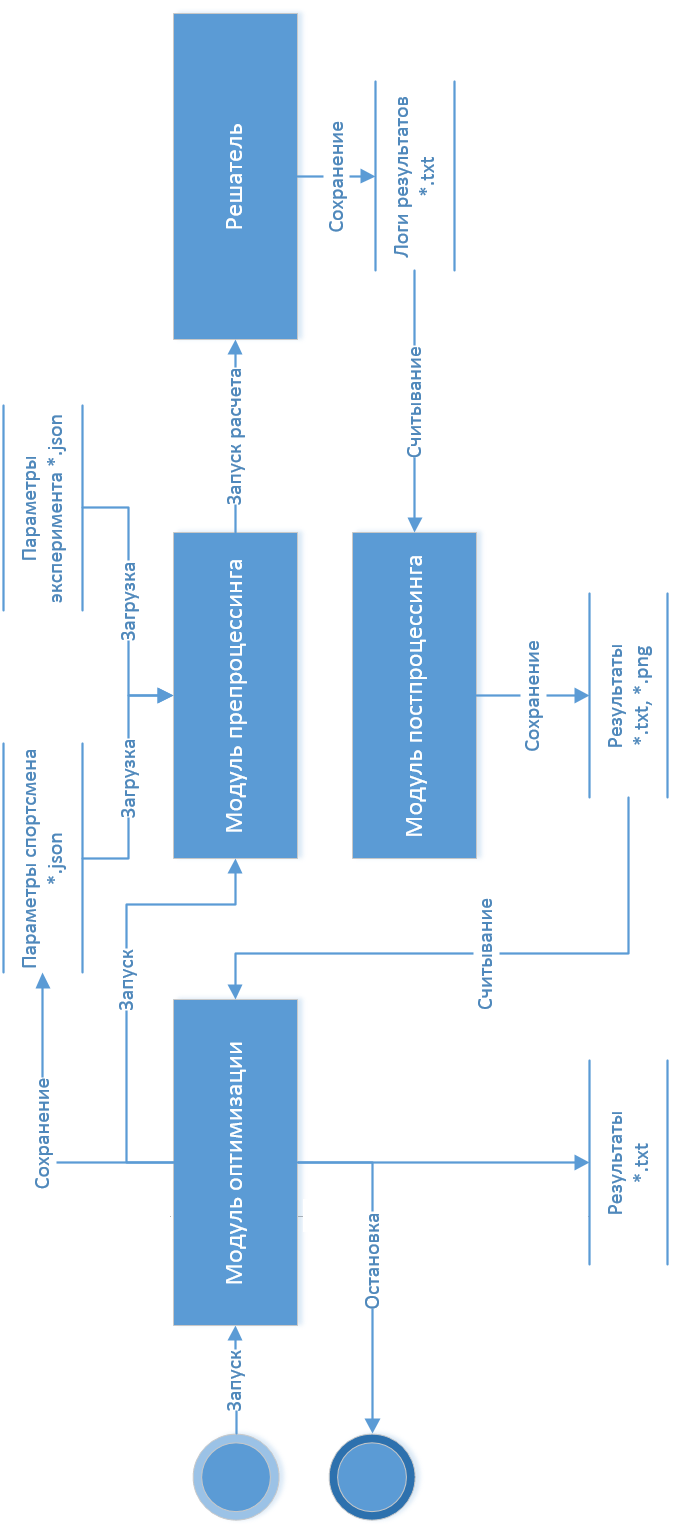
\includegraphics[scale=0.6]{pc5.png}
	\caption{Общая структура программного комплекса} 
	\label{fig:soft_muscle}
\end{figure}
Модуль оптимизации реализован на языке Python с использованием библиотек Scipy, Pandas, Numpy. В данном модуле используются реализация алгоритмов глобальной оптимизации из библиотеки Scipy.optimize. Для расчета новой точки оптимизатор перезаписывает файл конфигурации спортсмена и запускает модуль препроцессинга. После завершения работы решателя и модуля постпроцессенга, оптимизатор считывает файлы результатов, на основе которых рассчитывает функцию потерь. Данный процесс повторяется в цикле до достижения сходимости идентифицируемых параметров модели. 

Алгоритм определения аэробного и анаэробного порогов был реализован в виде отдельного программного комплекса (десктопное приложение) для использования экспертами-физиологами в своей  повседневной работе. Пользовательский интерфейс реализован на языке JavaScript с использованием библиотек ElectronJS и D3, ядро алгоритма - на языке C\#. Помимо определения порогов в программный комплекс добавлен функционал для работы в ручном режиме (удобное отображение данных, различные варианты сглаживания, возможность выделения интервалов)(Рис.~\ref{fig:soft_gasvis}). 
\begin{figure}[!ht]
	\centering
	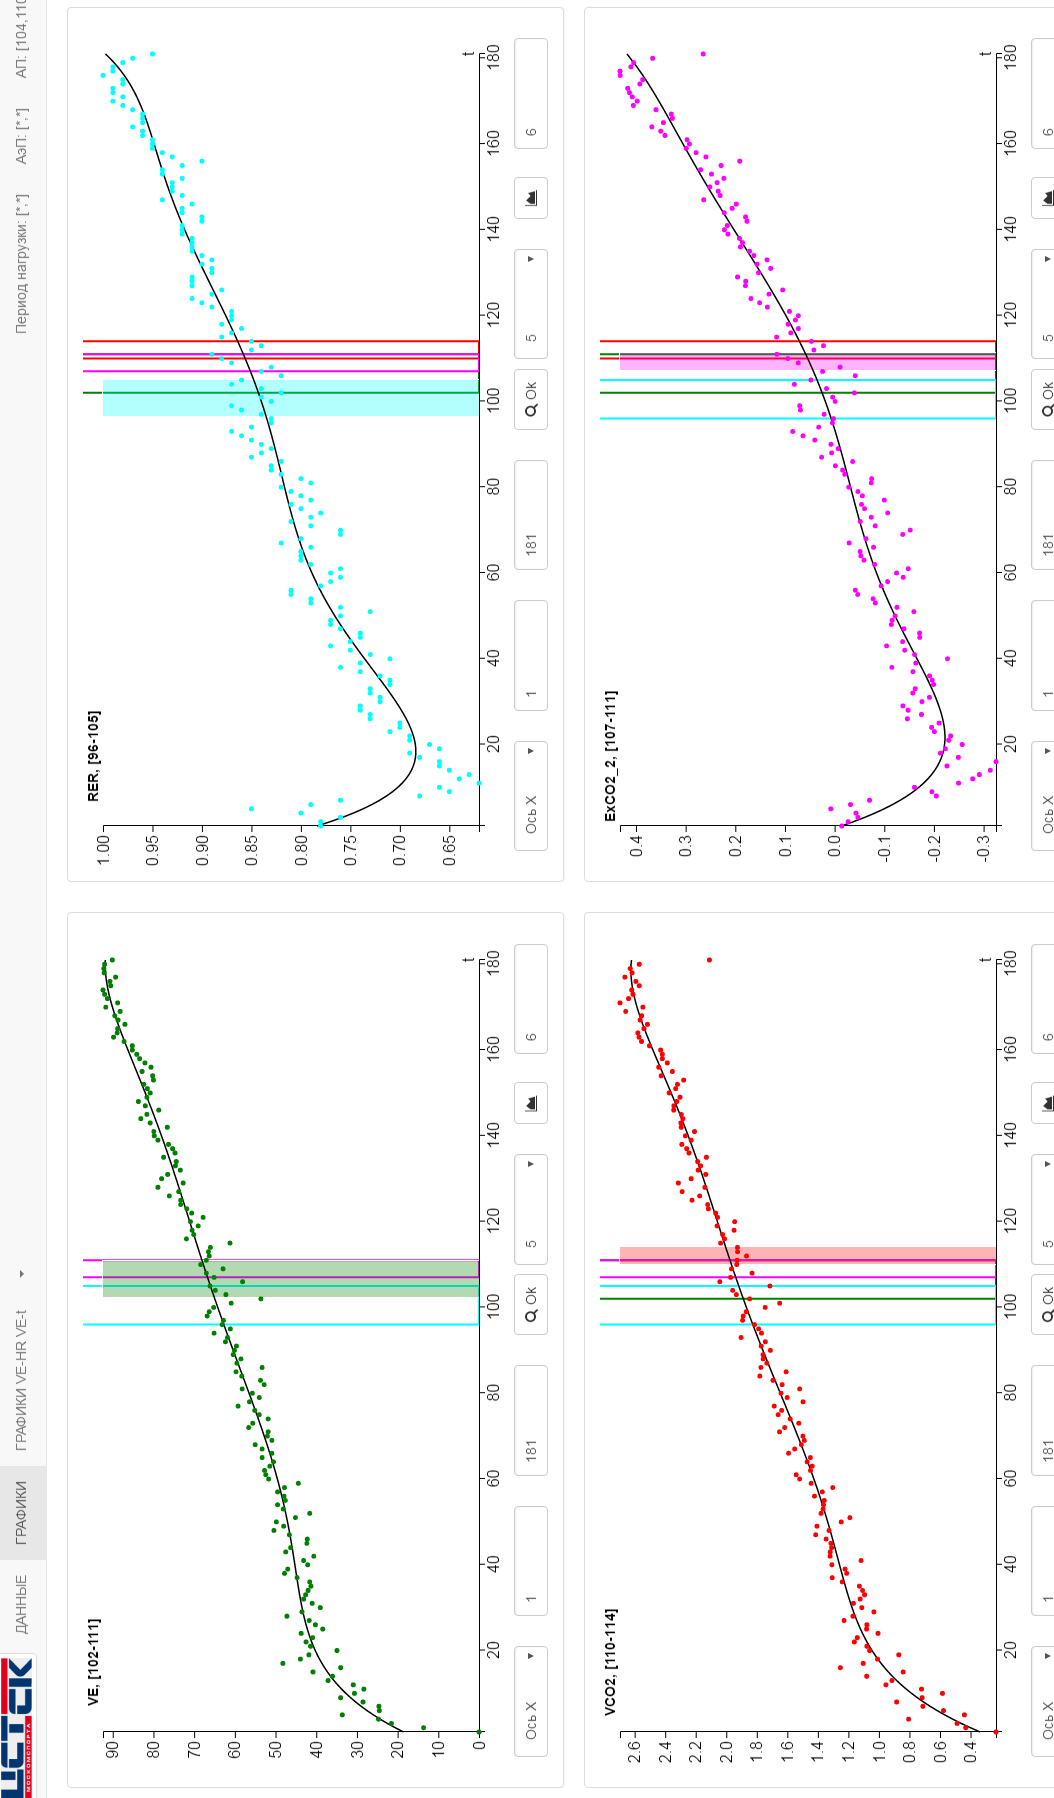
\includegraphics[scale=0.5]{gasvis.png}
	\caption{Пользовательский интерфейс программного комплекса для определения аэробного и анаэробного порогов} 
	\label{fig:soft_gasvis}
\end{figure}

\clearpage
\section{Резюме}
\begin{itemize}
\item 
Для описания транспорта газов в кровеносной системе используется модель, основанная на разделении системы на пять крупных отделов, соответствующих артериям тканей, головного мозга и легких, системным и легочным венам. Модель учитывает связывание $O_{2}$ гемоглобином и механизм поддержания кислотно-щелочного баланса в крови. 
\item
При физической нагрузке в модели учитываются механизмы производства и утилизации лактата (рассматривается переход от аэробного к анаэробному энергообмену), а также образование неметаболических излишек $CO_{2}$.
\item
Регуляция сердечного выброса и перераспределения кровотока между головным мозгом и тканями описывается эмпирической зависимостью от парциального давления $CO_{2}$ в системных артериях.
\item 
Для описания глобального газообмена в организме модель кровеносной системы и мышечного метаболизма дополняются усредненной моделью дыхательной системы.
\item
Регуляция параметров легочной вентиляции описывается эмпирической зависимостью от парциального давления $CO_{2}$, $O_{2}$ в системных артериях (периферические хеморецепторы) и $CO_{2}$ в артериях головного мозга (центральные хеморецепторы). 
\item
Модель сводится к решению 4х жестких систем ОДУ. Для численного расчета применялся A,L~-- устойчивый метод третьего порядка аппроксимации из семейства схем Обрешкова, а также итерационной процедуре совместного расчета газообмена с легкими и моделями регуляции.
\item
Неизвестные параметры модели идентифицируются по результатам тестов с возрастающей нагрузкой. Для минимизации функции ошибок применяется алгоритм дифференциальной эволюции ~--  стохастический алгоритм глобальной оптимизации.
\item 
Модель кровеносной системы и мышечного метаболизма реализована в виде программного комплекса с использованием абстрактной модели и архитектура, описанная в разделе \ref{lung:soft}. Для расчета 900 сек. нагрузочного теста на двух ядерном Intel Core i3-2100 3.10GHz, Windows 7-64, 16Gb RAM требовалось в среднем 10 секунд. Был добавлен дополнительный модуль оптимизации на языке Python.
\item
Значение анаэробного порога(используется в модели мышечного метаболизма) определяется с помощью робастного алгоритма по нескольким физиологическим показателям. Алгоритм был реализован в виде отдельного программного комплекс на языках JavaScript и C\#. Данный комплекс был внедрен в ЦСТиСК Москомспорта.  

\end{itemize}